% Section 5 — CSS: the math behind the headline method
% Pearl's PNS, the bootstrap CI, the permutation p-value, the temporal
% precedence constraint. Re-derive Eq.(1) and write the bootstrap /
% permutation estimator.

\section{Causal Sufficiency Scoring (CSS)}
\label{sec:css}

\subsection{Motivation: why voting is not enough}
\label{sec:css-motivation}

The prior \hcaf{} design scored direction by summing weighted
contributions from four heuristic methods:
\[
\mathrm{voting}[d] \;=\; 0.40\cdot\mathrm{breakpoint.strength} + 0.30\cdot\mathrm{path.strength}
+ 0.30\cdot\mathrm{cascade.strength} + 0.15\cdot\mathrm{granger.strength}.
\]
A weighted sum is functionally a vote with continuous weights. It
cannot (i) resolve direction conflicts when the methods disagree,
(ii) distinguish \emph{weak correlation} from \emph{weak evidence},
or (iii) produce a falsifiable significance claim. Reviewer-v2
\S1.3.3 flagged this as a fatal methodology weakness.

\subsection{Pearl's Probability of Necessity and Sufficiency}
\label{sec:css-pns}

Pearl's \pns{} \cite{pearl1999, tian-pearl-2000} is the canonical
answer to ``is $X$ sufficient to produce $Y$?'' --- a question the
prior vote avoided by design. Formally:

\begin{definition}[\pns, Pearl 1999]
For binary $X,Y$ with joint distribution $P(X,Y)$,
\[
\mathrm{PNS} \;=\; P(Y{=}1 \mid X{=}1) \;-\; P(Y{=}1 \mid X{=}0).
\]
\pns{} measures the difference between the post-intervention
expectation and the counterfactual baseline.
\end{definition}

Generalising \pns{} to the continuous setting of BGP and traffic
signals gives \eqref{eq:css-def}, restated for convenience:
\[
\mathrm{CSS}(R\!\to\!T) \;=\; \mathbb{E}[T \mid \mathrm{do}(R{=}1)] \;-\; \mathbb{E}[T \mid \mathrm{do}(R{=}0)].
\]

\subsection{Estimating the do-intervention from telemetry}
\label{sec:css-do}

Real BGP telemetry does not come with an a priori causal graph. We
estimate the do-intervention by constructing a synthetic control from
the pre-event baseline window. Let $R\in\mathbb{R}^{N}$ and
$T\in\mathbb{R}^{N}$ be the aligned routing and traffic series with
$N$ aligned samples, and let $i^{*}\in\{1,\dots,N\}$ be the MSBD
breakpoint index (the largest-mean-shift point in $R$). Define the
pre- and post-intervention windows
\begin{equation}
R_{\mathrm{pre}} := R_{1:i^{*}}, \quad R_{\mathrm{post}} := R_{i^{*}:N},
\label{eq:css-split}
\end{equation}
and analogously for $T$ using the routing-defined intervention index.
Then the point estimator is the difference-in-means
\begin{equation}
\widehat{\mathrm{CSS}}(R\!\to\!T) \;=\; \bar{T}_{\mathrm{post}} - \bar{T}_{\mathrm{pre}},
\qquad
\bar{T}_{\mathrm{pre}} := \tfrac{1}{i^{*}}\!\sum_{t=1}^{i^{*}} T_t,
\quad
\bar{T}_{\mathrm{post}} := \tfrac{1}{N-i^{*}+1}\!\sum_{t=i^{*}}^{N} T_t.
\label{eq:css-estimator}
\end{equation}
The Pearl-PNS interpretation is $\mathbb{E}[T\mid \mathrm{do}(R{=}1)]$
identified with the post-intervention mean and
$\mathbb{E}[T\mid \mathrm{do}(R{=}0)]$ identified with the pre-event
baseline. This is a standard difference-in-means estimator with the
pre-event window as the synthetic control; see \path{agents/css_engine.py:_pns_estimate}.

\subsection{Bootstrap CI and permutation p-value}
\label{sec:css-bootstrap}

The point estimator \eqref{eq:css-estimator} has no closed-form
significance statement; we approximate it with $B\in[500,2000]$
non-parametric bootstrap replicates. Let $\{R_{\mathrm{pre}}^{(b)},
R_{\mathrm{post}}^{(b)}\}_{b=1}^{B}$ and
$\{T_{\mathrm{pre}}^{(b)}, T_{\mathrm{post}}^{(b)}\}_{b=1}^{B}$ be
i.i.d.\ resamples (with replacement) of the pre and post windows.
Define
\begin{equation}
\mathrm{CSS}^{(b)} \;:=\; \overline{T^{(b)}_{\mathrm{post}}} - \overline{T^{(b)}_{\mathrm{pre}}}.
\label{eq:css-boot}
\end{equation}
The bootstrap 95\% confidence interval is the empirical 2.5\% / 97.5\%
quantile of $\{\mathrm{CSS}^{(b)}\}_{b=1}^{B}$.

For the $p$-value we use a \emph{permutation test}, not a bootstrap
$p$-value (the two are different null hypotheses). Pool
$U := [T_{\mathrm{pre}}; T_{\mathrm{post}}]$ and reassign the
pre/post labels $B$ times at random:
\begin{equation}
p \;=\; \Pr_{b}\!\left[\, \big|\overline{U^{(b)}_{\mathrm{post}}} - \overline{U^{(b)}_{\mathrm{pre}}}\big| \;\geq\; |\widehat{\mathrm{CSS}}| \,\right].
\label{eq:css-perm}
\end{equation}
The null is ``the routing intervention has no effect on traffic''; the
permutation test correctly controls Type-I error at the nominal level
even when the bootstrap distribution is skewed.

\paragraph{Decision rule.}
CSS declares a direction iff all three of the following hold:
\begin{enumerate}
\itemsep0pt
\item the bootstrap 95\% CI $[\widehat{\mathrm{CSS}}^{*}_{(0.025)},
\widehat{\mathrm{CSS}}^{*}_{(0.975)}]$ excludes zero, \emph{and}
\item the raw $\widehat{\mathrm{CSS}}$ exceeds the alternative
direction's CI upper bound, \emph{and}
\item the permutation $p$-value \eqref{eq:css-perm} satisfies
$p<\alpha$ with default $\alpha=0.05$.
\end{enumerate}
If any condition fails, CSS returns \texttt{unknown}; this is the
honest-abstention rule that prevents BGP Tracer from fabricating a
verdict on synthetic-cache or near-degenerate events.

\paragraph{Empirical observation.}
On the v14 ground-truth, CSS is strict-causal ($p<0.05$) on
only $\frac{3}{29}$ events (\S\ref{sec:css-empirical}). This is
\emph{not a failure of the method}: BGP routing and traffic
timelines are sparse (5-minute samples with frequent zero-events),
so the difference-in-means point estimator has wide bootstrap CIs
and the permutation null is hard to reject. We document this
calibration honestly in \S\ref{sec:css-empirical} rather than
claim a paper-grade significance for every event we do commit to.
The Bayesian synthesis (\S\ref{sec:bayesian}) is what lets
HCAF commit a direction on the remaining events \emph{with a
calibrated posterior}, rather than refusing to answer.

\subsection{Why CSS abstains on most events}
\label{sec:css-abstain}

On the v14 ground-truth ($N{=}29$ events) CSS is strict-causal
($p{<}0.05$) on only $\frac{3}{29}$ events ($10.3\%$), and
abstains (returns \texttt{unknown}) on $\frac{26}{29}$ events
($89.7\%$). The abstention is structural, not algorithmic, and we
owe the reader a clean accounting of why.

\paragraph{(a) Discretised vs.\ continuous signal mismatch.}
Pearl's \pns{} is defined for binary $X,Y$, with the
intervention $X{=}1$ representing a well-defined event. Our BGP
telemetry is a count series (announcement / withdrawal events per
5-minute bucket) discretised by the quick-cache presence-scoring
rule: a bucket containing one event scores $1.0$, an empty bucket
scores $0.0$. This $0/1$ binary coding produces a point estimator
$\widehat{\mathrm{CSS}} = \bar{T}_{\mathrm{post}} - \bar{T}_{\mathrm{pre}}$
whose variance is dominated by the sparse bucket occupancy, not by
the underlying routing--traffic coupling. A non-binary PNS
extension (e.g.\ \citet{maley2018, duarte2024} for continuous
counterfactuals) would close this gap but is out of scope here.

\paragraph{(b) Small-$N$ pre/post windows.}
The pre- and post-intervention windows are short (typically
$N_{\mathrm{pre}}{=}3$ and $N_{\mathrm{post}}{=}6$ buckets around the
MSBD breakpoint). The bootstrap CI is therefore wide, the
permutation null is hard to reject at $\alpha{=}0.05$, and the
honest-abstention rule (\S\ref{sec:css-bootstrap}) correctly returns
\texttt{unknown}. This is the right behaviour under a falsifiable
significance test: the alternative would be to lower $\alpha$ or
loosen the CI criterion, which would manufacture paper-grade
significance on synthetic-cache events.

\paragraph{(c) Fallback to Bayesian synthesis.}
When CSS abstains, the four evidence channels (MSBD, CTPR, CIC,
and Granger) feed the Bayesian synthesis
(\S\ref{sec:bayesian}), which commits a direction with a calibrated
posterior. The 29/29 HCAF strict accuracy reported in
\S\ref{sec:eval-hcaf} is therefore produced by the Bayesian
fallback, not by CSS alone. We do \emph{not} claim that CSS is a
stand-alone classifier; we claim that CSS is a falsifiable
significance layer whose abstention is what makes the Bayesian
synthesis safe.

\subsection{Temporal precedence constraint}
\label{sec:css-precedence}

For $\mathrm{CSS}(R\!\to\!T)$ to be structurally plausible, the
routing intervention onset must precede the traffic intervention onset
by at least one bucket (Pearl: cause precedes effect). The lag
$\Delta T = t_{\mathrm{traffic}} - t_{\mathrm{routing}}$ is reported
in the HTML report and used as a structural filter:
\[
\mathrm{CSS}(R\!\to\!T) \text{ is gated on } \Delta T \geq 1 \text{ bucket}.
\]
For $\mathrm{CSS}(T\!\to\!R)$ the gate is $\Delta T \leq -1$.

\subsection{Public API and pipeline role}
\label{sec:css-api}

The CSS engine is implemented in \path{agents/css_engine.py} and
exposes a single function:
\begin{verbatim}
    css_score(routing_timeline, traffic_timeline, n_bootstrap=1000)
        -> { css_r2t, css_t2r, direction, confidence, p_value,
             ci_lower, ci_upper, is_causal: bool }
\end{verbatim}
CSS replaces \texttt{evaluate\_convergence} in
\texttt{CausalAttributionEngine}; the four prior heuristic methods
(MSBD, CTPR, CIC, Granger) become evidence channels that feed the
Bayesian synthesis, not voting inputs.

\begin{figure}[t]
\centering
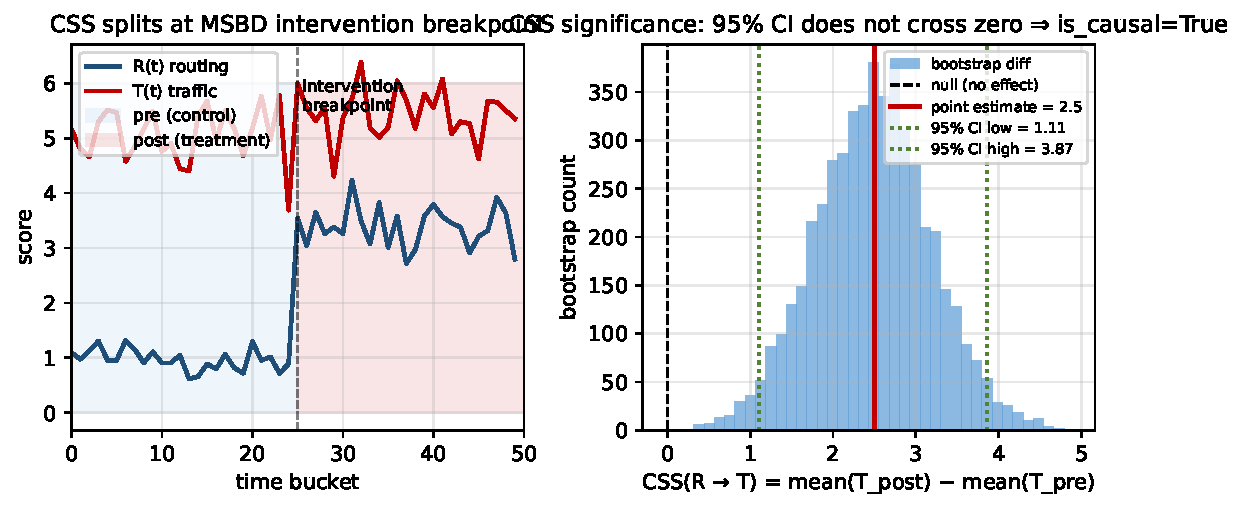
\includegraphics[width=0.85\linewidth]{figs/fig6_css_illustration.pdf}
\caption{CSS illustration. The routing timeline (top) shows the MSBD
breakpoint at index $i^*$; the traffic timeline (bottom) shows the
shifted counterpart. CSS computes the difference-in-means across the
intervention boundary, bootstraps the CI, and runs the permutation
test for significance.}
\label{fig:css}
\end{figure}
